\documentclass[11pt, oneside]{amsart}
\usepackage{geometry}
\geometry{a4paper,top=1in,bottom=1in}
\usepackage[parfill]{parskip}
\usepackage{graphicx}
\usepackage{amssymb}
\pagestyle{empty}

\newcommand{\problem}[2]{\section*{#1: #2}}
\newcommand{\solution}[0]{{\sc solution}}

\title{Tages Anzeiger math problems}

\begin{document}
\maketitle

The Zürich daily {\em Tages Anzeiger} has a math column edited by
Dmitrij Nikolenkov of ETH. Here are some problems (translated by me
from German to English) and my solutions.

\vspace{2em}\hrule\vspace{2em}

\problem{2024-05-02}{Overlapping squares}

Three squares with the given side lenghts overlap as follows:

\begin{figure}[!h] 
    \centering
    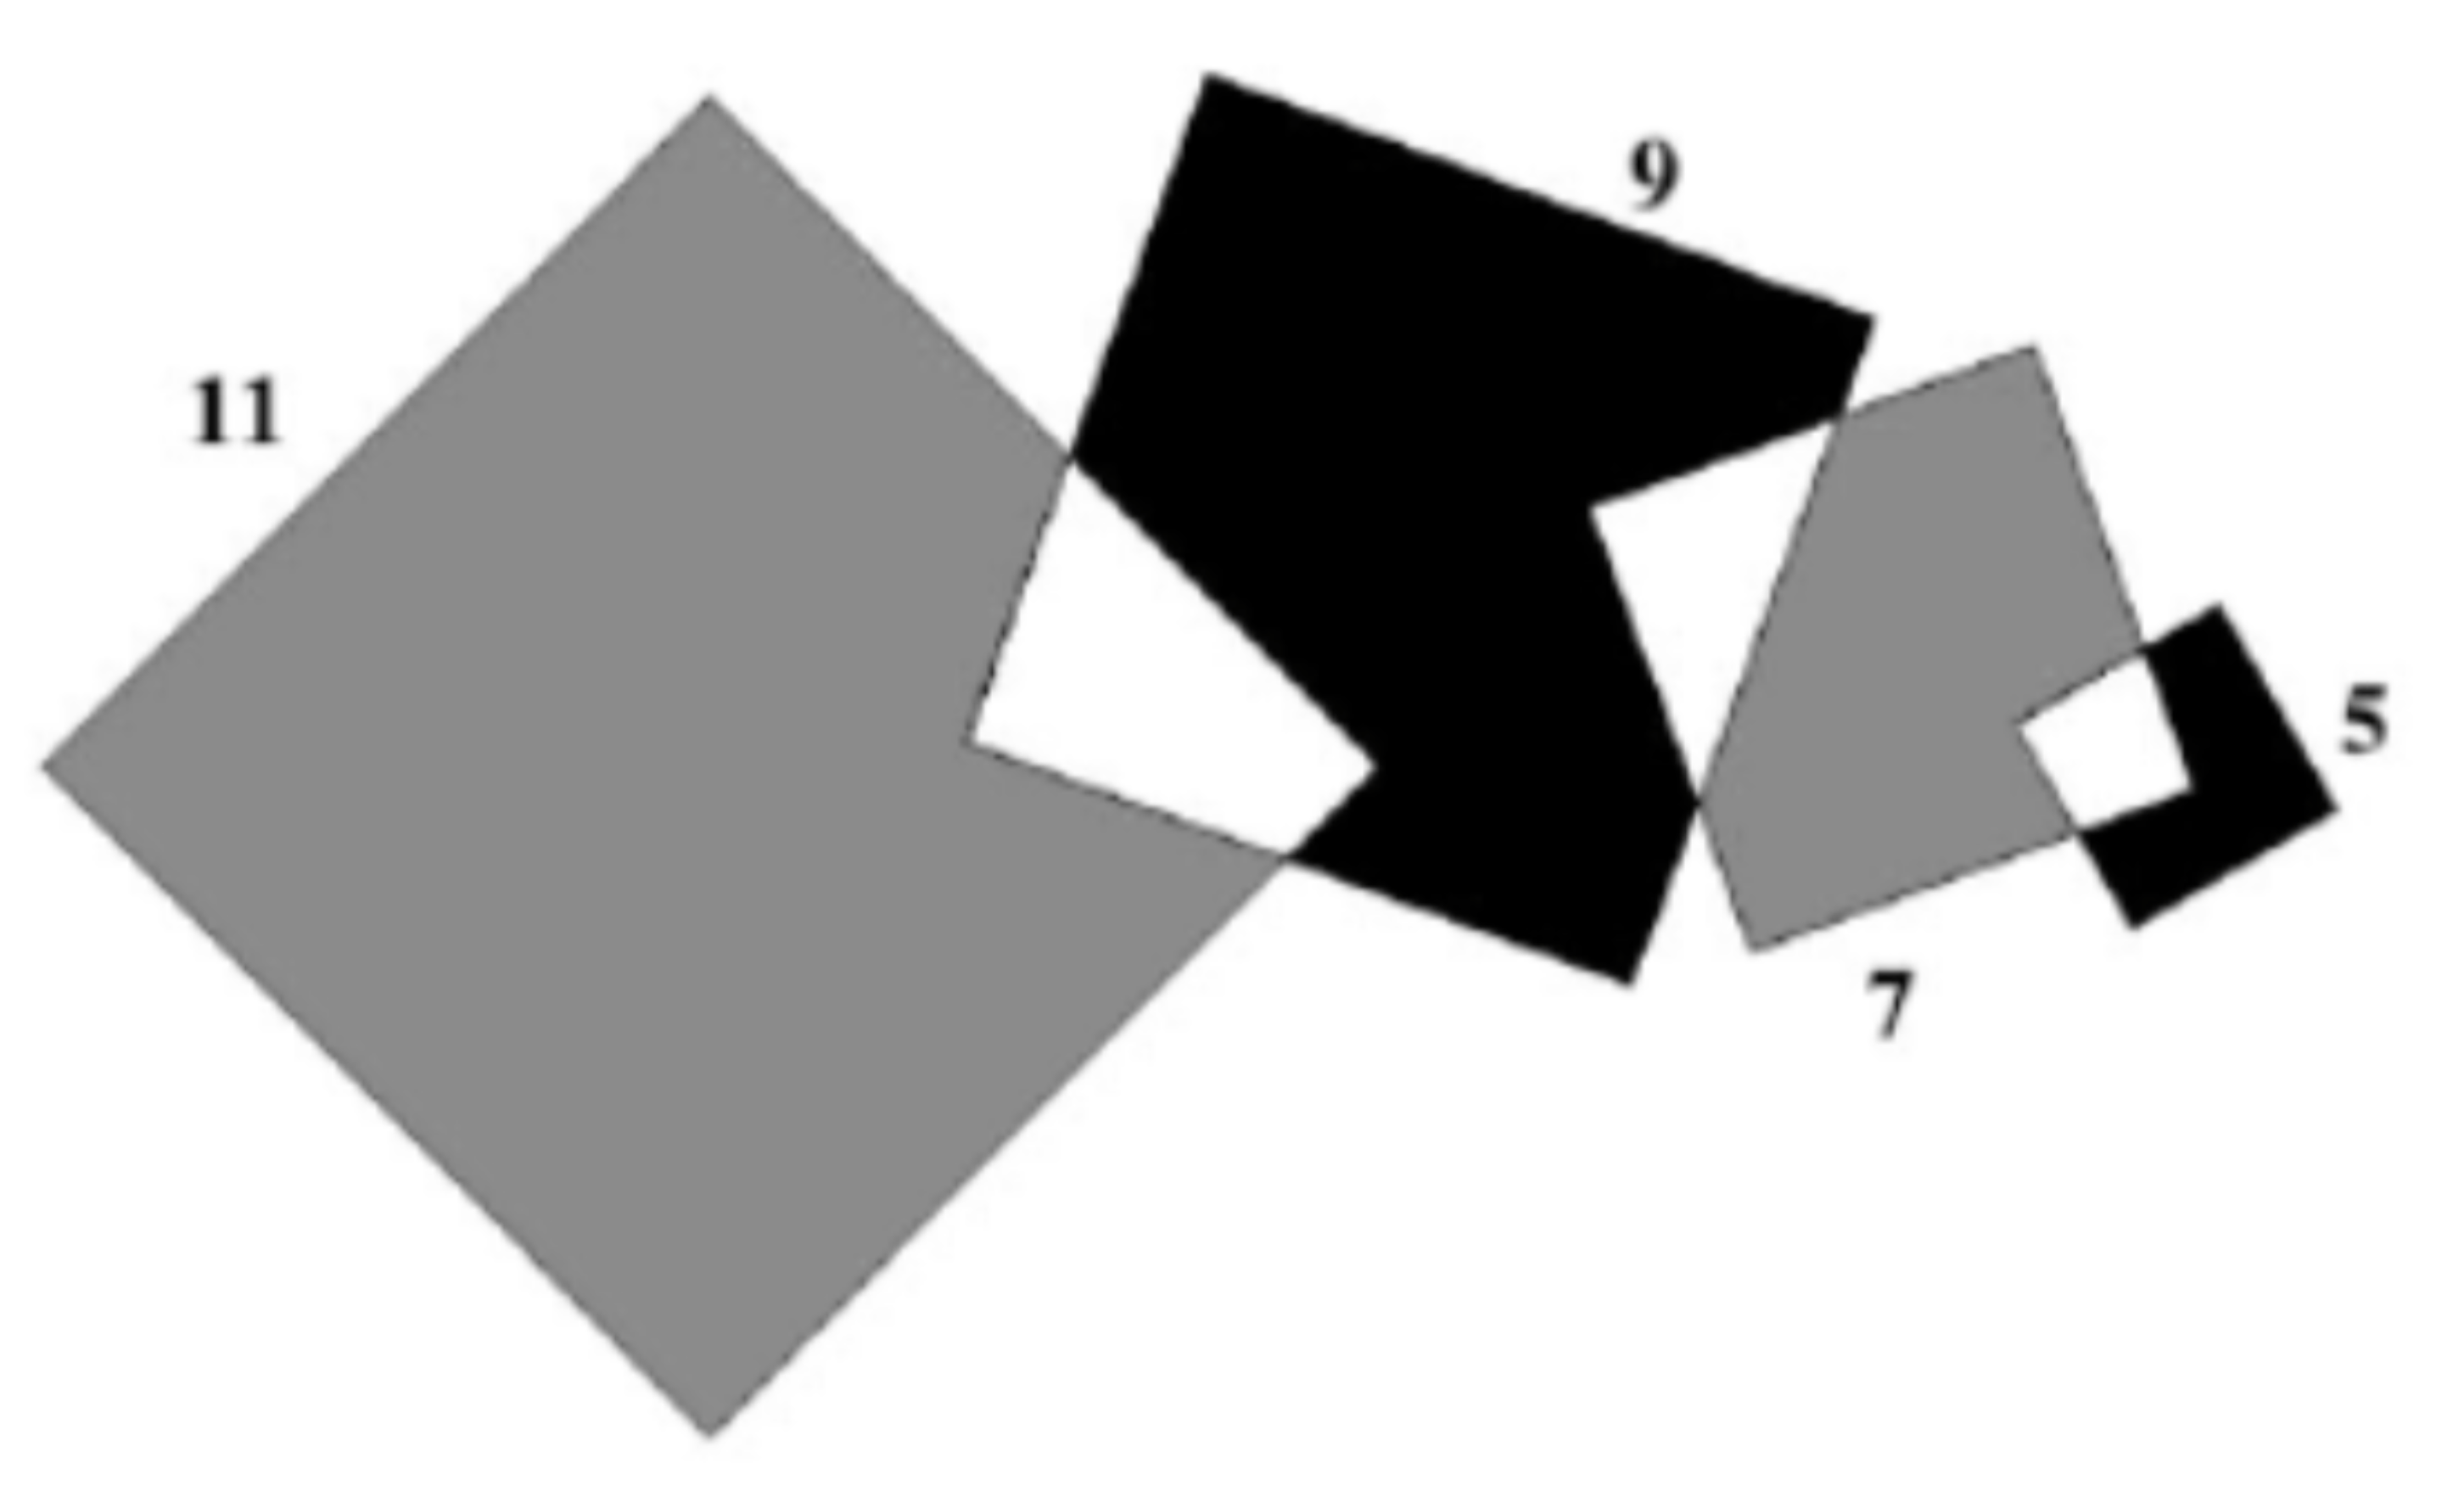
\includegraphics[width=0.5\textwidth]{squares.png}
\end{figure}

The gray surface is twice as large as the black surface. What is the area of the white surface?

\solution

The area of gray + white is $11^2 + 7^2 = 170$. The area of black + white is $9^2+5^2 = 106$.

Let $w$ be the white area. Then $170 - w =  2(106-w)$ and it follows that $w = 42$.

\newpage
\problem{2024-05-02}{Interesting boxes}

The width and height of a box (a rectangular parallelepiped) are two consecutive
positive integers. Its depth is equal to the product of those two integers.
Prove that the diagonal of such a box is always an integer.

\solution

Denote the bottom face of the box by the vertices $ABCD$ and let the corresponding
vertices of the top face be $WXYZ$. The front face is given by $ABXW$.

Then, given the problem description, $|AB| = x$, $|BX| = x+1$, $|BC| = x(x+1)$.

Define a diagonal $AC$ across the bottom face, and let $d_1 = |AC|$.
By the Pythagorean theorem,
\[ d_1^2 = x^2 + x^2(x+1)^2 = x^4 + 2x^3 + 2x^2. \]

A diagonal of the parallelepiped is $AY$. Let $d_2 = |AY|$.
By the Pythagorean theorem,
\begin{align*}
	 d_2^2 &= d_1^2 + (x+1)^2 \\
           &= x^4 + 2x^3 + 3x^2 + 2x + 1 \\
           &= (x^2 + x + 1)^2
\end{align*}
Since $x$ is an integer, $d_2 = (x^2 + x +1)$ is an integer also.

\newpage
\problem{2024-05-16}{Numbers game}

Alf and Bettina play the following game. They take turns to write {\em different} digits
from left to right until they have a 9-digit number. Alf starts (and finishes). If the resulting number is divisible by 4, Alf wins, otherwise Bettina wins.
Do Alf or Bettina have a winning strategy? If so, what does it look like?

\solution

A number of two or more digits is divisible by 4 iff its last two digits
are divisible by 4. (A number whose last two digits are $00$ is divisible by
4 because 100 is divisible by 4.)

The two-digit numbers with non-repeating digits that are divisible by 4 are:
\[ 04~08~12~16~20~24~28~32~36~40~48~52~56~60~64~68~72~76~80~84~92~96 \]

Bettina can have a winning strategy. She can use her first three turns
to ensure that 2, 4, and 6 are used (if Alf has not already chosen
them). As a result, only the following divisible-by-4 sequences can appear
in the last two digits:
\[ 08~80 \]

On her fourth turn, Bettina can pick any remaining odd number. (Since Alf
has had four turns, there is guaranteed to be at least one.)

Now, even if 0 and 8 are still available, Alf cannot choose a final digit
such that the last two digits are 08 or 80. Bettina wins.

\newpage
\problem{2024-05-16}{Fractions}

Find three different irreducible fractions with numerators and denominators
not equal to 1 whose sum is an integer and the sum of the reciprocals is
also an integer. There are many solutions.

\solution

I could not find an analytical way to solve this problem so I wrote a short program
to find all combinations (with replacement) of irreducible fractions $<1$ with both numerator
and denominator in $[2, 49]$ and test them for the desired property. See {\tt fractions.py}
in the current directory. The results:

\begin{align*}
10/27 + 2/27   + 5/9\\
3/28  + 15/28  + 5/14\\
2/11  + 3/11   + 6/11\\
4/5   + 4/5    + 2/5\\
\end{align*}

\newpage
\problem{2024-06-27}{Digit sum times 2024}

Let $Q(n)$ be the sum of digits of a natural number $n$. For all $n$, $Q(2n) \leq 2Q(n)$.

Find a number $n$ such that $Q(n) = 2024 \cdot Q(3n)$.

\solution

Restating the problem, we know that for all $n$:
\[ \frac{Q(2n)}{Q(n)} \leq 2 \]
and we want some $n$ such that:
\[ \frac{Q(3n)}{Q(n)} = \frac{1}{2024} \leq 2 \]

Let's use the notation $x\{k\}y$ to denote a natural number in base 10 where the digit $x$ is repeated $k$ times
and followed by the digit $y$.

Playing around a bit to build intuition, for all positive $k$, $2(9\{k\}9) = 19\{k\}8$ and
\[ \frac{Q(19\{k\}8)}{Q(9\{k\}9)} = \frac{1+9k+8}{9k+9} = 1\]

Similarly, $2(1\{k\}) = 2\{k\}$ and
\[ \frac{Q(2\{k\})}{Q(1\{k\})} = 2\]

Intuitively, we want to find some increasing sequence of numbers $n_i$ that contain a repeating pattern of digits
such that $Q(n_i)$ grows much more quickly than $Q(3n_i)$ as the pattern of digits increases in length.
Can we find a $3n$ that consists mostly of 0s while $n$ does not?

The simplest pattern for which this is true is numbers of the form $n = 3\{k\}y$ with $y \in \{ 4, 5, 6 \}$. Then
$3n = 10\{k\}z$, where $z \in \{ 2, 5, 8 \}$, respectively.

We may be onto something! Let's build a table:

\begin{table}[h!]
\centering
\begin{tabular}{|c|c|c|c|}
	\hline
	$n$      & $3\{k\}4$    & $3\{k\}5$    & $3\{k\}6$ \\
	\hline
	$3n$     & $10\{k\}2$   & $10\{k\}5$   & $10\{k\}8$ \\
	\hline
	$Q(n)$   & $3k+4$       & $3k+5$       & $3k+6$ \\
	\hline
	$Q(3n)$  & $3$          & $6$          & $9$ \\
	\hline
\end{tabular}
\end{table}

$\frac{3k+4}{3} = 2024$ has no integer solution (for any $m$, $3m-4 \mod 3 = 2$).

$\frac{3k+5}{6} = 2024$ has no integer solution (for any $m$, $6m-5 \mod 3 = 1$).

But $\frac{3k+6}{9} = 2024$ does have an integer solution ($9m-6 \mod 3 = 0$). $k = 6070$,
so $n = 3\{6070\}6$ (and $3n = 10\{6070\}8$).


\end{document}  